% exercise sheet with header on every page for math or close subjects
\documentclass[12pt]{article}
\usepackage[utf8]{inputenc} 
\usepackage{latexsym} 
\usepackage{multicol}
\usepackage{fancyhdr}
\usepackage{amsfonts} 
\usepackage{amsmath}
\usepackage{amssymb}
\usepackage{enumerate}
\usepackage{listings}
\usepackage{graphicx}
\usepackage{float}


% Shortcuts for bb, frak and cal letters
\newcommand{\E}{\mathbb{E}}
\newcommand{\V}{\mathbb{V}}
\renewcommand{\P}{\mathbb{P}}
\newcommand{\N}{\mathbb{N}}
\newcommand{\R}{\mathbb{R}}
\newcommand{\C}{\mathbb{C}}
\newcommand{\Z}{\mathbb{Z}}
\newcommand{\Pfrak}{\mathfrak{P}}
\newcommand{\Pfrac}{\mathfrak{P}}
\newcommand{\Bfrac}{\mathfrak{P}}
\newcommand{\Bfrak}{\mathfrak{B}}
\newcommand{\Fcal}{\mathcal{F}}
\newcommand{\Ycal}{\mathcal{Y}}
\newcommand{\Bcal}{\mathcal{B}}
\newcommand{\Acal}{\mathcal{A}}


% Formatierung
\topmargin -2cm 
\textheight 24cm
\textwidth 16.0 cm 
\oddsidemargin -0.1cm

\setlength{\parindent}{0pt}  % !!!!!!! Hier werden leerzeilen erlaubt ohne dass Latex automatisch einrueckt! !!!!!!! %


\graphicspath{ {images/} }


\begin{document}

% Titel
%\title{\textsc{Hacking}\\ \textsc{Abgabe 0}\\{ \normalsize Gruppe X \hfill Daniel Schäfer (2549458)\\ \hfill Anderer}}
%\maketitle  

% alternativer Titel
\noindent
{\Large \textbf{High-level Computer Vision}} \hfill \textbf{06.06.2016}\\
{\Large \textbf{Exercise 5}} 
\raggedleft \hfill Guillermo Reyes (2556018)\\
\hfill Daniel Schaefer (2549458)\\
\hfill Marc Tonsen (2537359)\\
\hfill Dominik Weber (2548553)\\

\pagenumbering{gobble}
\raggedright


\section*{Code Annotations}




\section{Data Augmentation}

\begin{enumerate}[a)]
        \setcounter{enumi}{1}
    \item 
        %TODO
        % flip occurs in batch and thus the flipped pictures are different after every get_batch, results in overall 'more' training data
\end{enumerate}


\section{Mean Image Substraction}

\begin{enumerate}[a)]
        \setcounter{enumi}{1}
    \item 
        We should not use both sets at once to compute the mean, because in that case the test data would have an impact on our training which would compromise the evaluation. Instead only the image-mean of the training data should be substracted from both the training data and the test data. The test-data should not be transformed differently than the training-data because the distribution of the test data must not be altered differently than the training data to ensure the equality of both the testing and training data distribution. 
    \item
        The best validation error decreased from 0.72 to 0.64 in our Plot.
        \begin{figure}[H]
            \centering
                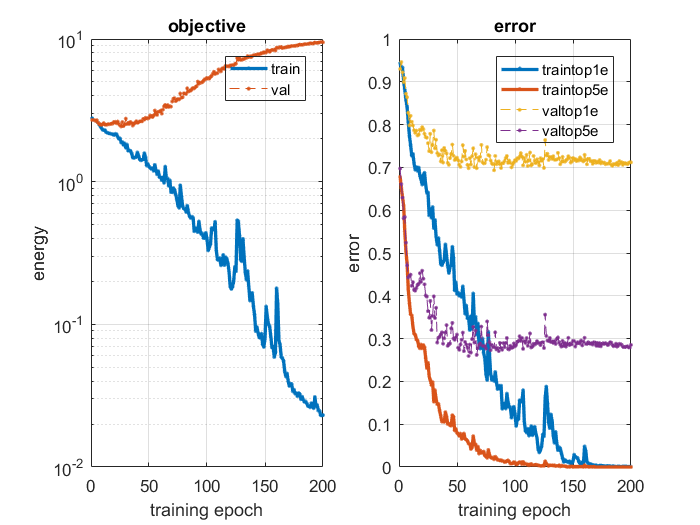
\includegraphics[width=0.9\textwidth]{Plots/init_plot_epo_200.png}
                \caption{without using mean-image substraction}
        \end{figure}
        \begin{figure}[H]
            \centering
                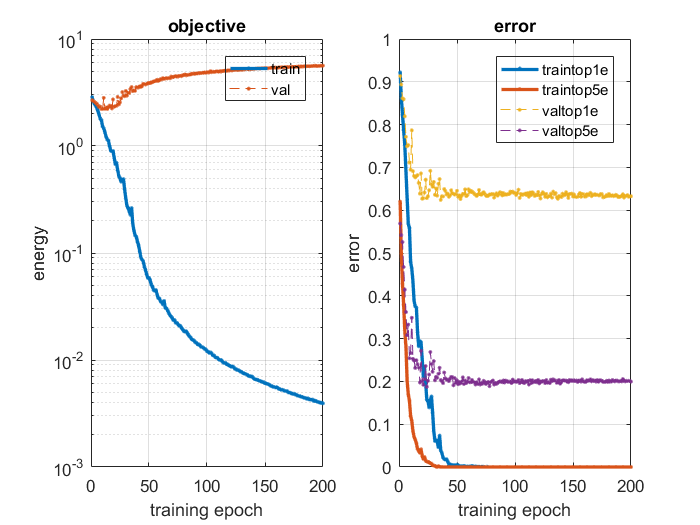
\includegraphics[width=0.9\textwidth]{Plots/q2_plot_epo_200.png}
                \caption{with using mean-image substraction}
        \end{figure}
        Also the validation error seems to decrease faster.\\
        Similar to the previous cases the training error quickly decreases further while the validation error remains rougly on the same level which indicates overfitting
\end{enumerate}


\section{Dropout}

\begin{enumerate}[a)]
    \item 
        Dropout works very close in spirit to Random Forsts. Random Forests consist of a set of decision trees. Each single decision tree is very prone to overfitting to the training-data. However the random forst simply picks the average result out of all decision trees which effectifely cancels out the overfitting to a high amount. Dropout intuitively does the same: it trains several subsets of the network on the training-data and ''takes the average'' of them. 
    \item
        Of cause not! At test-time we want to utilize the full power of the network. Discarding parts of it doesn't make sense.
    \item
        %TODO nicht eindeutig eins besser, haengt von daten ab. Dann noch spezifisch schreiben wie es bei uns aussieht und was wie gut wird/ist
        Using our Implementation a dropout of 50\% resulted in the lowest error (testing 100epochs) with around 66\% Error 
        \begin{figure}[H]
            \centering
                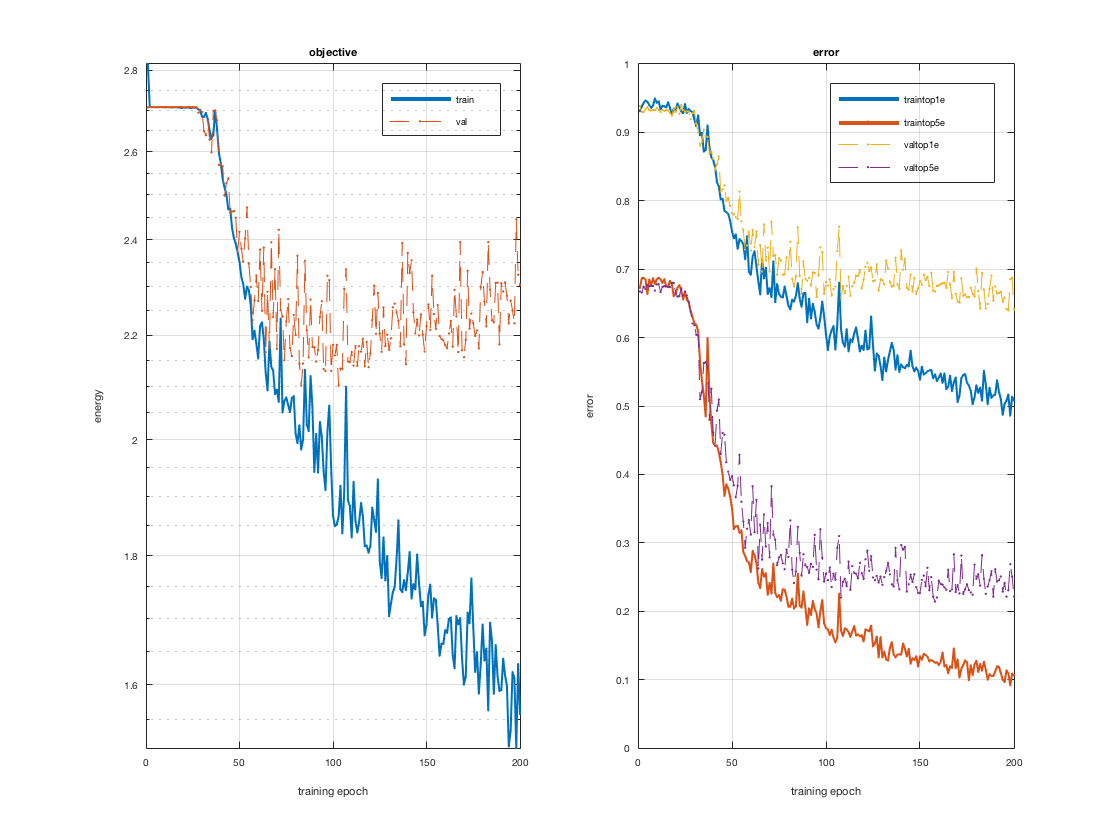
\includegraphics[width=0.9\textwidth]{Plots/3_50_200.png}
                \caption{using a Dropout of 50\%}
        \end{figure}
        followed by 25\% dropout resulting in 68\% Error 
        \begin{figure}[H]
            \centering
                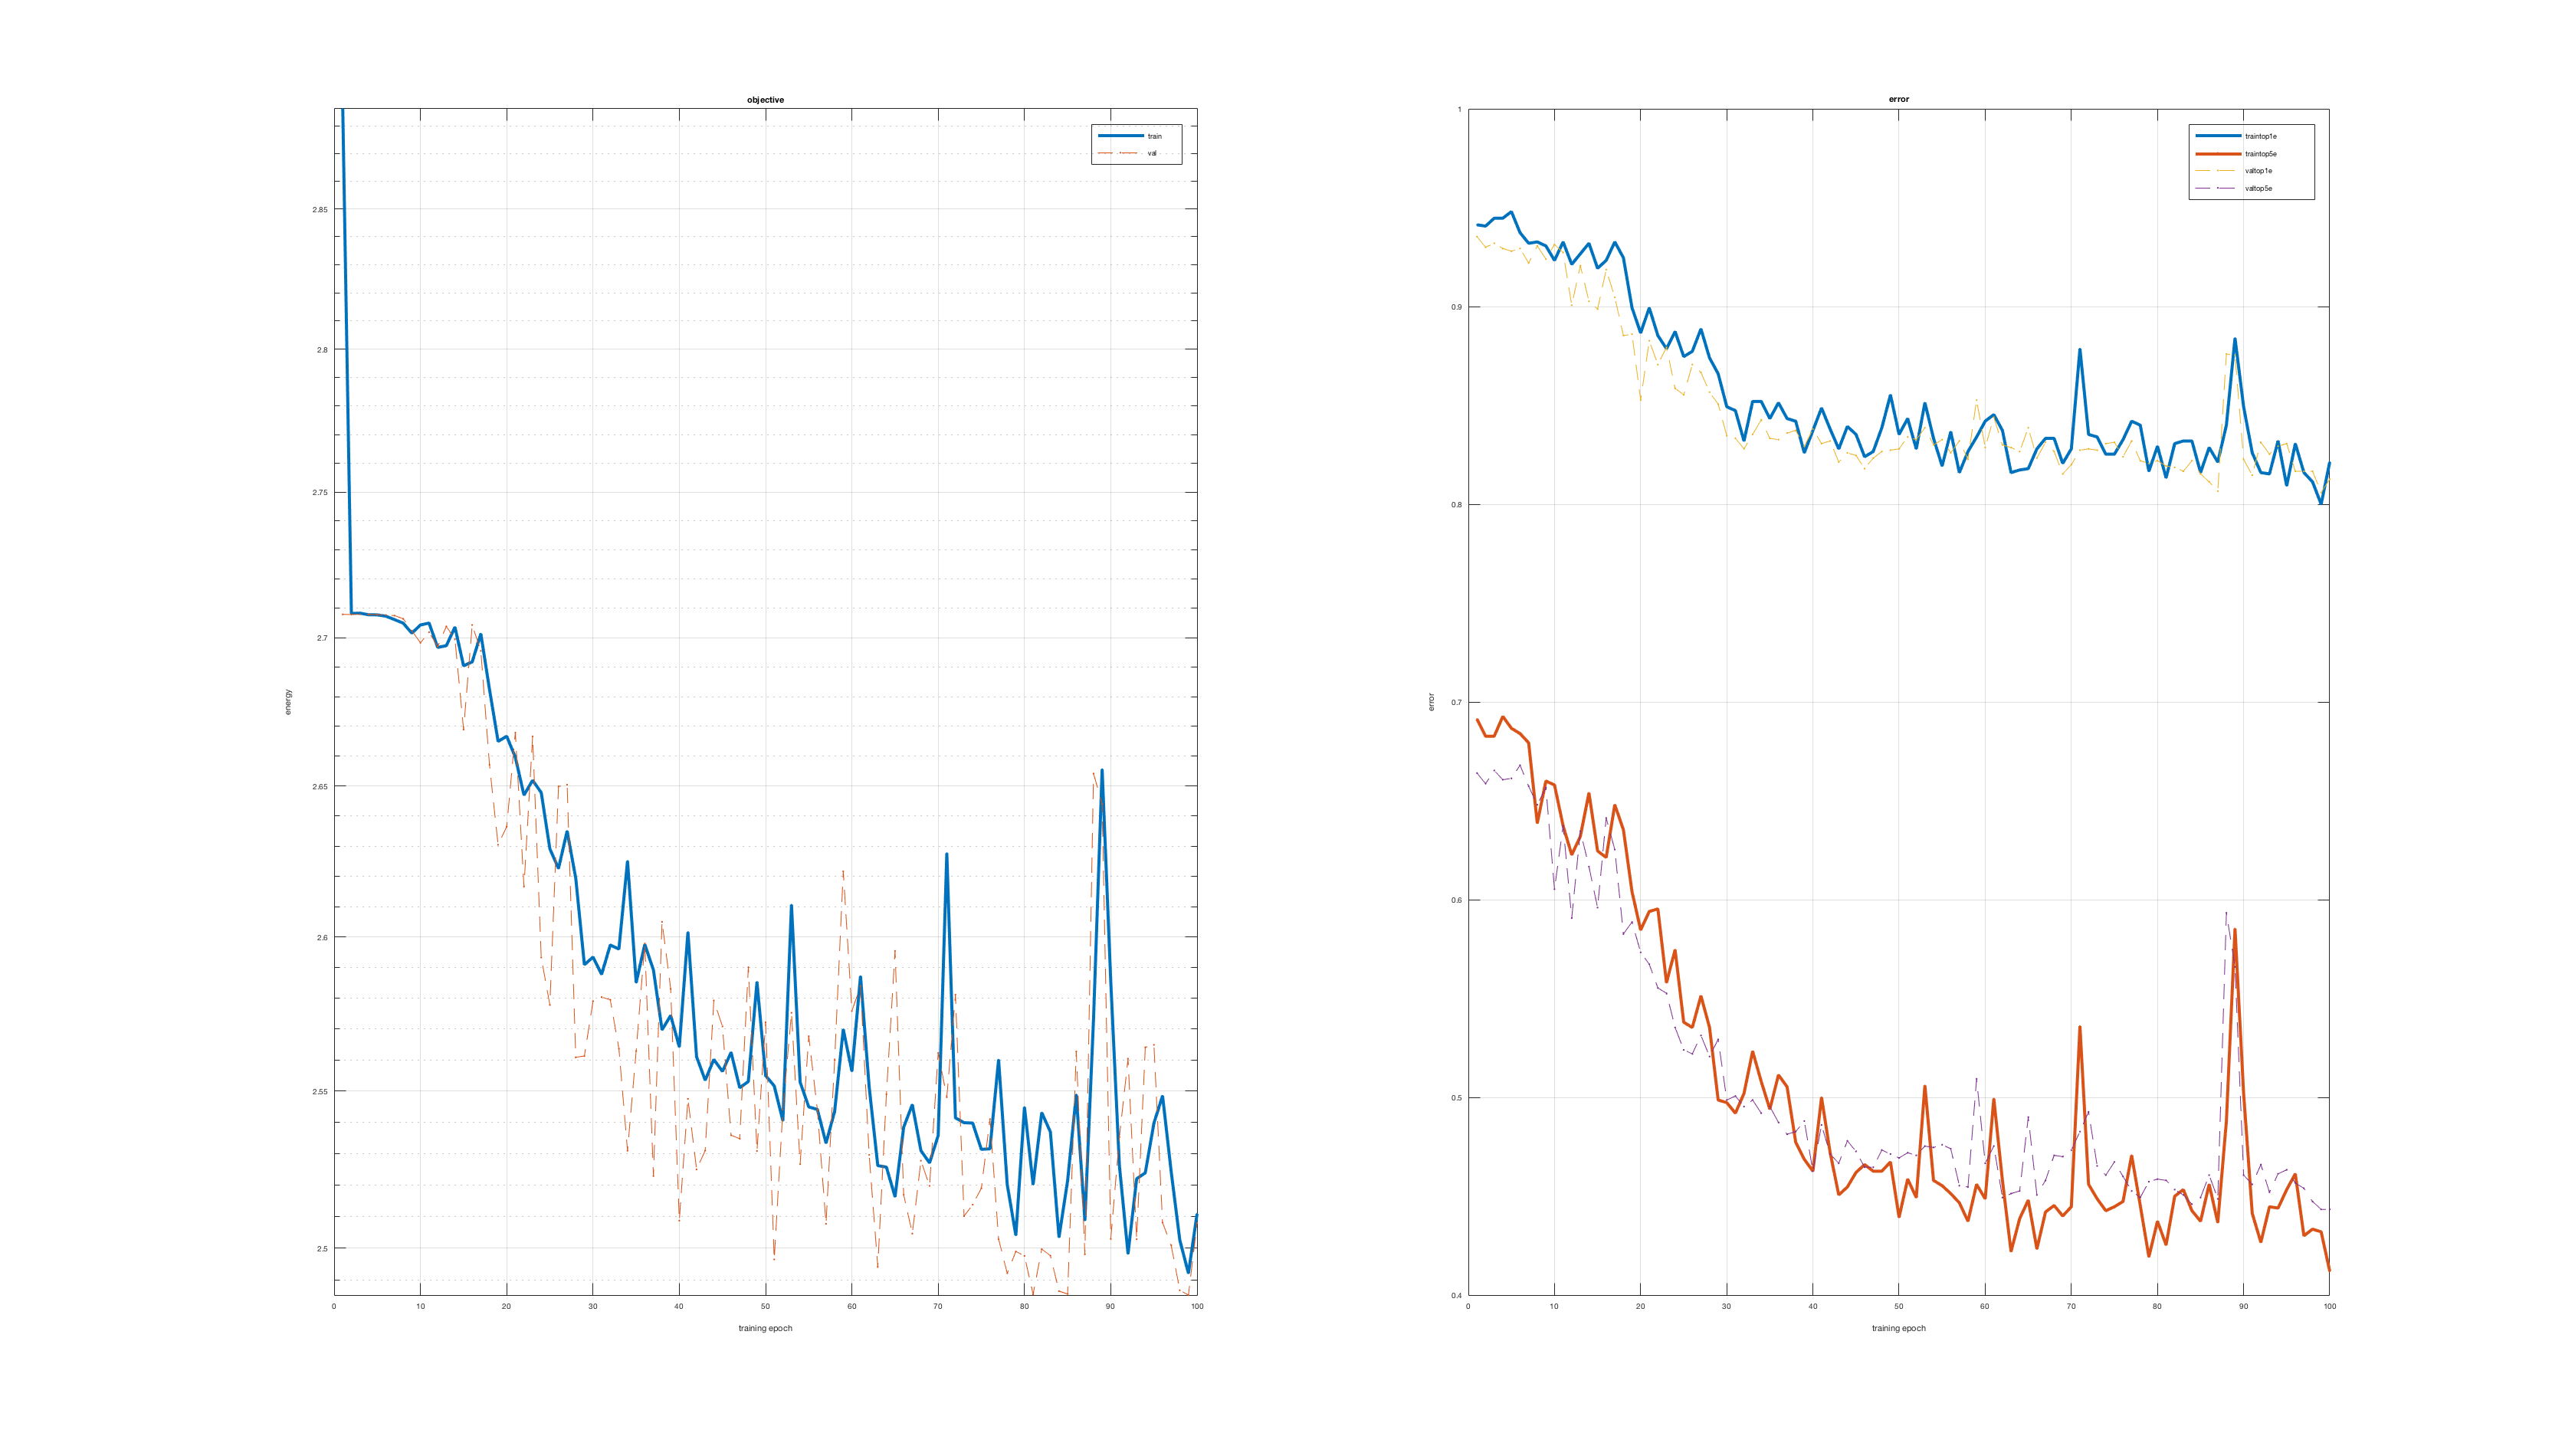
\includegraphics[width=0.9\textwidth]{Plots/3_75_100.png}
                \caption{using a Dropout of 25\%}
        \end{figure}
        and 75\% Dropout resulting in around 80\% Error.
        \begin{figure}[H]
            \centering
                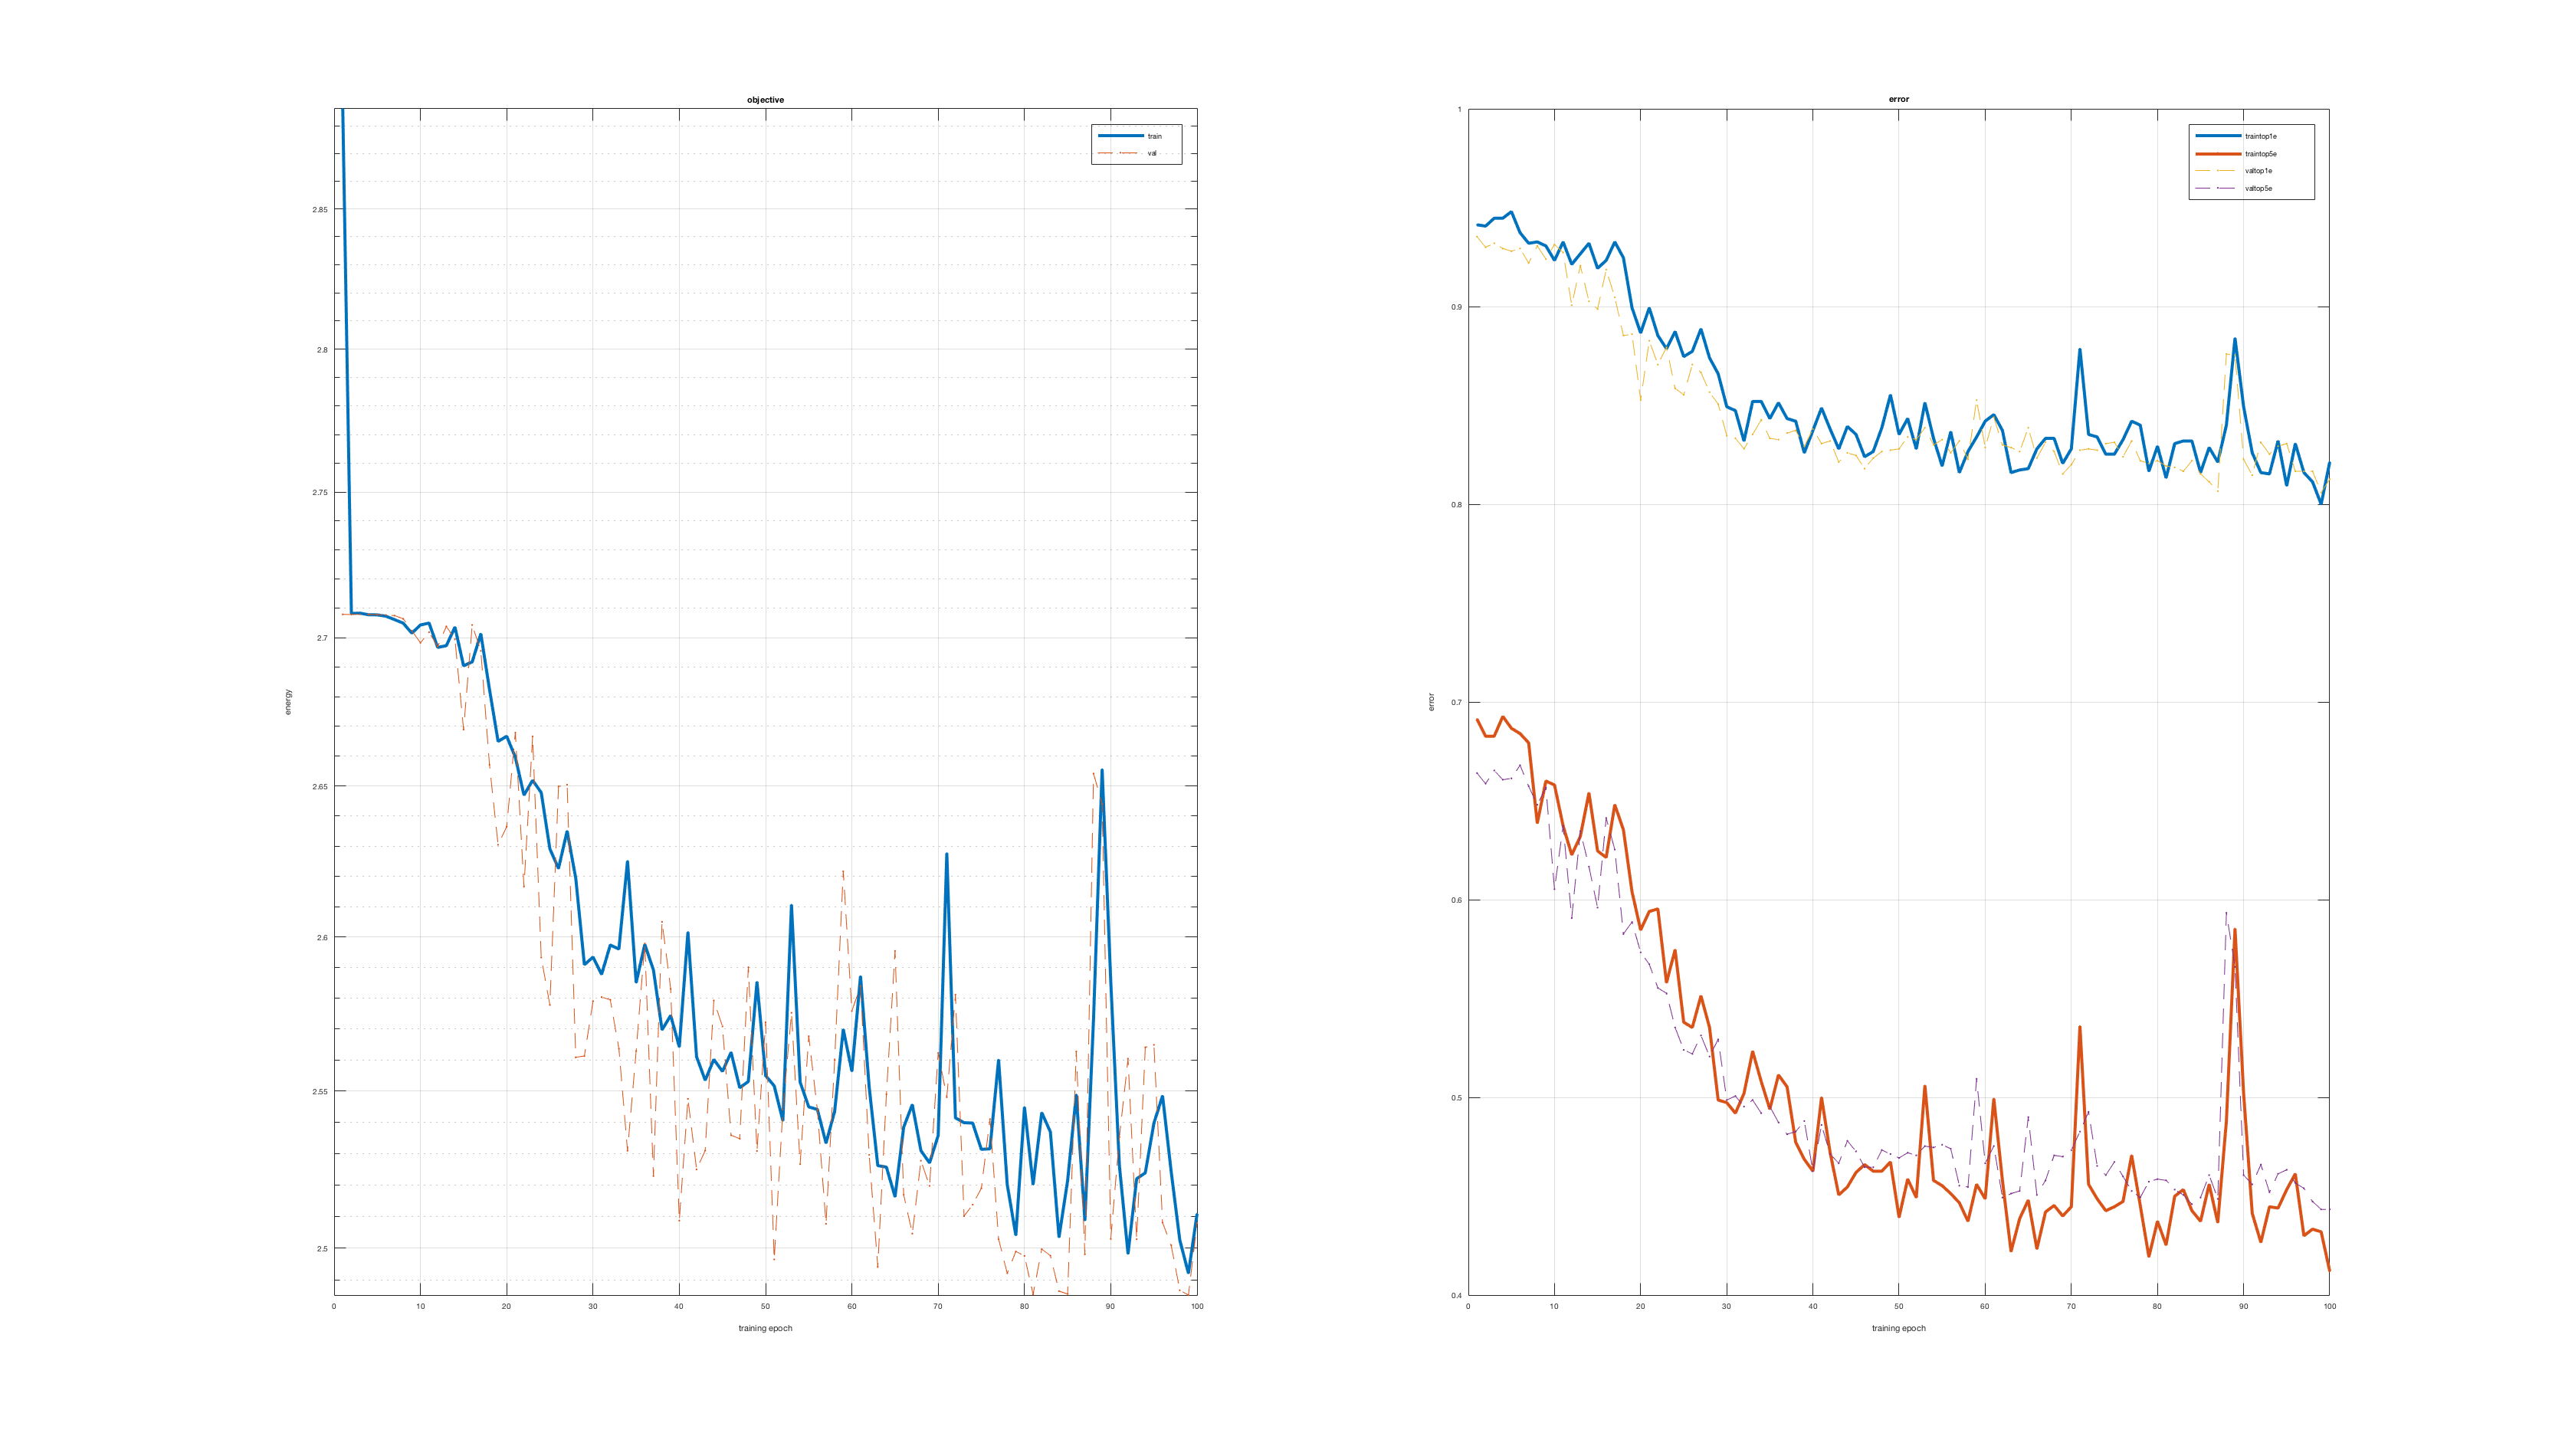
\includegraphics[width=0.9\textwidth]{Plots/3_75_100.png}
                \caption{using a Dropout of 75\%}
        \end{figure}
\end{enumerate}


\newpage
\section{CNN with more Layers and Tricks}

        \begin{figure}[H]
            \centering
                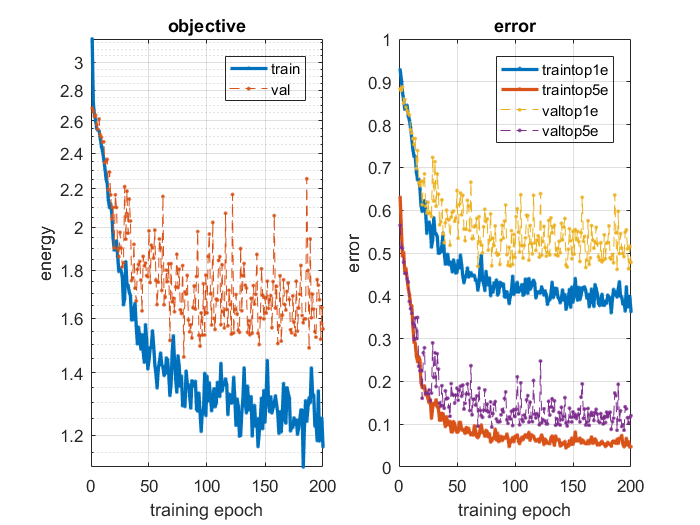
\includegraphics[width=0.9\textwidth]{Plots/q4_plot_epo_200.png}
                \caption{our Result using all the optimizations meantioned}
        \end{figure}
        We are achieving an Error rate of only 48\%, which is significant improvement to the 0.72\% without our optimizations!
        \begin{figure}[H]
            \centering
                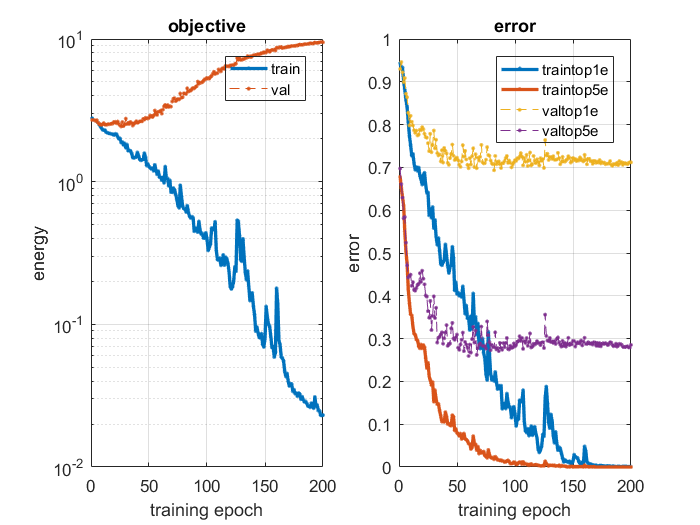
\includegraphics[width=0.9\textwidth]{Plots/init_plot_epo_200.png}
                \caption{our Result using no optimizations}
        \end{figure}



\end{document}
